%% abtex2-modelo-projeto-pesquisa.tex, v-1.9.6 laurocesar
%% Copyright 2012-2016 by abnTeX2 group at http://www.abntex.net.br/ 
%%
%% This work may be distributed and/or modified under the
%% conditions of the LaTeX Project Public License, either version 1.3
%% of this license or (at your option) any later version.
%% The latest version of this license is in
%%   http://www.latex-project.org/lppl.txt
%% and version 1.3 or later is part of all distributions of LaTeX
%% version 2005/12/01 or later.
%%
%% This work has the LPPL maintenance status `maintained'.
%% 
%% The Current Maintainer of this work is the abnTeX2 team, led
%% by Lauro César Araujo. Further information are available on 
%% http://www.abntex.net.br/
%%
%% This work consists of the files abntex2-modelo-projeto-pesquisa.tex
%% and abntex2-modelo-references.bib
%%

% ------------------------------------------------------------------------
% ------------------------------------------------------------------------
% abnTeX2: Modelo de Projeto de pesquisa em conformidade com 
% ABNT NBR 15287:2011 Informação e documentação - Projeto de pesquisa -
% Apresentação 
% ------------------------------------------------------------------------ 
% ------------------------------------------------------------------------

\documentclass[
	% -- opções da classe memoir --
	12pt,				% tamanho da fonte
	openright,			% capítulos começam em pág ímpar (insere página vazia caso preciso)
	oneside,			% para impressão em recto e verso. Oposto a oneside
	a4paper,			% tamanho do papel. 
	% -- opções da classe abntex2 --
	%chapter=TITLE,		% títulos de capítulos convertidos em letras maiúsculas
	%section=TITLE,		% títulos de seções convertidos em letras maiúsculas
	%subsection=TITLE,	% títulos de subseções convertidos em letras maiúsculas
	%subsubsection=TITLE,% títulos de subsubseções convertidos em letras maiúsculas
	% -- opções do pacote babel --
	english,			% idioma adicional para hifenização
	french,				% idioma adicional para hifenização
	spanish,			% idioma adicional para hifenização
	brazil,				% o último idioma é o principal do documento
	]{abntex2}

% ---
% PACOTES
% ---

% ---
% Pacotes fundamentais 
% ---
\usepackage{lmodern}			% Usa a fonte Latin Modern
\usepackage[T1]{fontenc}		% Selecao de codigos de fonte.
\usepackage[utf8]{inputenc}		% Codificacao do documento (conversão automática dos acentos)
\usepackage{indentfirst}		% Indenta o primeiro parágrafo de cada seção.
\usepackage{color}				% Controle das cores
\usepackage{graphicx}			% Inclusão de gráficos
\usepackage{microtype} 			% para melhorias de justificação
\usepackage[table,xcdraw]{xcolor}
% ---

% ---
% Pacotes adicionais, usados apenas no âmbito do Modelo Canônico do abnteX2
% ---
\usepackage{lipsum}				% para geração de dummy text
% ---

% ---
% Pacotes de citações
% ---
\usepackage[brazilian,hyperpageref]{backref}	 % Paginas com as citações na bibl
\usepackage[alf]{abntex2cite}	% Citações padrão ABNT

% --- 
% CONFIGURAÇÕES DE PACOTES
% --- 

% ---
% Configurações do pacote backref
% Usado sem a opção hyperpageref de backref
\renewcommand{\backrefpagesname}{Citado na(s) página(s):~}
% Texto padrão antes do número das páginas
\renewcommand{\backref}{}
% Define os textos da citação
\renewcommand*{\backrefalt}[4]{
	\ifcase #1 %
		Nenhuma citação no texto.%
	\or
		Citado na página #2.%
	\else
		Citado #1 vezes nas páginas #2.%
	\fi}%
% ---

% ---
% Informações de dados para CAPA e FOLHA DE ROSTO
% ---
\titulo{Análise Criteriosa de Um Sistema - \textit{Instagram}}
\autor{
	Antônio F. de Carvalho$^{1}$, Diego F. Sousa Lima$^{1}$\\
	Diego de S. Vasconcelos$^{1}$, Marcio Silvano$^{1}$
	\\
	$^{1}$Curso Bacharelado em Sistemas de Informação -- UFPI\\
	\texttt{\{antonio007023, diegofernando5672\}@gmail.com}\\
	\texttt{\{diegosousa.33, marcinho944\}@hotmail.com}
}

\local{Picos -- PI}
\data{2017}
\instituicao{%
  Universidade Federal do Piauí
  \par
  Curso Bacharelado em Sistemas de Informação
  }
% O preambulo deve conter o tipo do trabalho, o objetivo, 
% o nome da instituição e a área de concentração 
\preambulo{O objetivo geral deste trabalho é documentar todo
	o processo de análise do aplicativo \textit{Instagram} sob a ótica da IHC para a disciplina de Interação Humano-Computador
	sob a orientação do professor Frank Cesar Lopes Veras}
% ---

% ---
% Configurações de aparência do PDF final

% alterando o aspecto da cor azul
\definecolor{blue}{RGB}{41,5,195}

% informações do PDF
\makeatletter
\hypersetup{
     	%pagebackref=true,
		pdftitle={\@title}, 
		pdfauthor={\@author},
    	pdfsubject={\imprimirpreambulo},
	    pdfcreator={LaTeX with abnTeX2},
		pdfkeywords={abnt}{latex}{abntex}{abntex2}{projeto de pesquisa}, 
		colorlinks=true,       		% false: boxed links; true: colored links
    	linkcolor=blue,          	% color of internal links
    	citecolor=blue,        		% color of links to bibliography
    	filecolor=magenta,      		% color of file links
		urlcolor=blue,
		bookmarksdepth=4
}
\makeatother
% --- 

% --- 
% Espaçamentos entre linhas e parágrafos 
% --- 

% O tamanho do parágrafo é dado por:
\setlength{\parindent}{1.3cm}

% Controle do espaçamento entre um parágrafo e outro:
\setlength{\parskip}{0.2cm}  % tente também \onelineskip

% ---
% compila o indice
% ---
\makeindex
% ---

% ----
% Início do documento
% ----
\begin{document}

% Seleciona o idioma do documento (conforme pacotes do babel)
%\selectlanguage{english}
\selectlanguage{brazil}

% Retira espaço extra obsoleto entre as frases.
\frenchspacing 

% ----------------------------------------------------------
% ELEMENTOS PRÉ-TEXTUAIS
% ----------------------------------------------------------
% \pretextual

% ---
% Capa
% ---
\imprimircapa
% ---

% ---
% Folha de rosto
% ---
\imprimirfolhaderosto
% ---

% ---
% NOTA DA ABNT NBR 15287:2011, p. 4:
%  ``Se exigido pela entidade, apresentar os dados curriculares do autor em
%     folha ou página distinta após a folha de rosto.''
% ---

% ---
% inserir lista de ilustrações
% ---
\pdfbookmark[0]{\listfigurename}{lof}
\listoffigures*
\cleardoublepage
% ---

% ---
% inserir lista de tabelas
% ---
\pdfbookmark[0]{\listtablename}{lot}
\listoftables*
\cleardoublepage
% ---


% ---
% inserir o sumario
% ---
\pdfbookmark[0]{\contentsname}{toc}
\tableofcontents*
\cleardoublepage
% ---


% ----------------------------------------------------------
% ELEMENTOS TEXTUAIS
% ----------------------------------------------------------
\textual

% ----------------------------------------------------------
% Introdução
% ----------------------------------------------------------
\chapter*[Introdução]{Introdução}
\addcontentsline{toc}{chapter}{Introdução}

A interatividade do usuário e a avaliação individual por um conjunto específico de usuários  são atributos relacionados a usabilidade de um sistema. Estes parâmetros servem para definição dos critérios que presumem a qualidade de um \textit{software} de acordo com a norma ISO/IEC

Do mesmo modo, existem também os requisitos ergonomia, nos quais a ISO 9241-11 de 1998 define usabilidade como sendo: O grau em que um produto e usado por usuários específicos para atingir objetivos específicos com eficácia, eficiência e satisfação em um contexto de uso especifico.

Neste trabalho faremos uma visão do aplicativo \textit{Instagram} sob as óticas da Interação Humano-Computador. \textit{Instagram} é uma rede social online de compartilhamento de fotos e vídeos entre seus usuários, que permite aplicar filtros digitais e compartilhá-los em uma variedade de serviços de redes sociais, como \textit{Facebook}, \textit{Twitter}, \textit{Tumblr} e \textit{Flickr}. Originalmente, uma característica distintiva era a limitação as fotos para uma forma quadrada, semelhante ao \textit{Kodak Instamatic} e de câmeras \textit{Polaroid}, em contraste com a relação a proporção de tela de 16:9 tipicamente usada por câmeras de dispositivos móveis.

O \textit{Instagram} foi criado por Kevin Systrom e Mike Krieger e lançado em outubro de 2010. O serviço rapidamente ganhou popularidade, com mais de 100 milhões de usuários ativos em abril de 2012. O \textit{Instagram} é distribuído através da\textit{ Apple App Store}, \textit{Google Play} e \textit{Windows Phone Store}.

O presente documento se encontra organizado da seguinte maneira: na primeira seção é apresentada a lista de figuras; a seção 2 a lista de tabelas e, por conseguinte a lista de gráficos. Logo após damos início ao trabalho com seus perspectivo tópicos que serão abordados, e ultima seção traz as conclusões do trabalho.

% ----------------------------------------------------------
% Capitulo de textual  
% ----------------------------------------------------------
\chapter{Perspectiva da interação}

% Please add the following required packages to your document preamble:
% \usepackage[table,xcdraw]{xcolor}
% If you use beamer only pass "xcolor=table" option, i.e. \documentclass[xcolor=table]{beamer}
\begin{table}[h]
	\centering
	\caption{Perspectiva da Interação}
	\label{my-label}
	\begin{tabular}{|c|c|c|}
		\hline
		\rowcolor[HTML]{EFEFEF} 
		{\color[HTML]{000000} \textbf{Perspectiva}} & {\color[HTML]{000000} \textbf{Significado de interação}}                                    & {\color[HTML]{000000} \textbf{Fatores de qualidade mais evidentes}}                         \\ \hline
		Sistema                                     & Rede social                                                                                 & \begin{tabular}[c]{@{}c@{}}Interação com outros usuários\\ de imagens e vídeos\end{tabular} \\ \hline
		Ferramenta                                  & Envio de mídias sociais                                                                     & Entretenimento do usuário                                                                   \\ \hline
		Mídia                                       & \begin{tabular}[c]{@{}c@{}}Comunicação entre\\ os usuários\\ através de midias\end{tabular} & \begin{tabular}[c]{@{}c@{}}Qualidade da comunicação\\ alta\end{tabular}                     \\ \hline
	\end{tabular}
\end{table}

\chapter{Perspectiva de interface}

A interface de um sistema interativo compreende toda a porção do sistema com a qual o usuário mantem contato físico (motor ou perceptivo) ou conceitual durante a interação \cite{moran}. Ela e o único meio de contato entre o usuário e o sistema. Por isso, a grande maioria dos usuários acredita que o sistema é a interface com a qual entram em contato \cite{hix}.

\section{Contato FÍSICO}

O contato físico entre o usuário e o aplicativo \textit{Instagram} é feita, principalmente, por toques na tela do \textit{smartphone} já que a abordagem principal do sistema é uma aplicação móvel. Para esta finalidade o sistema se encontra em perfeito estado de comunicação entre usuário e sistema já que o tempo de resposta aos toques pode ser considerado rápido. O sistema também dispõe de uma versão voltada para a \textit{Web}. Neste caso, as entradas são feitas via mouse e teclado onde o usuário pode interagir com o sistema sendo que suas saídas são exibidas via monitor.

\section{Contato CONCEITUAL}

O contato conceitual do aplicativo \textit{Instagram} orienta o usuário para suas determinadas funções, para isso vários artifícios são usados. O mais claro consiste em fazer breves descrições das funcionalidades (Figura \ref{instaprivate}) quando o usuário faz o primeiro uso. Outro forma de direcionamento está nos ícones distribuídos pela tela em todos os ambientes do aplicativo, fazendo que o usuário tenha uma noção básica da serventia das ações.

\begin{figure}[htb]
	\caption{\label{instaprivate}Exemplo de descrição para auxílio do usuário}
	\begin{center}
		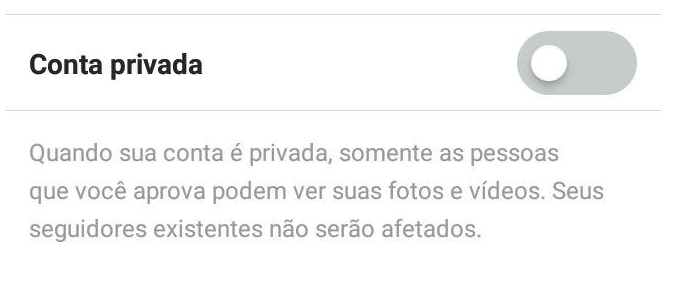
\includegraphics[scale=0.4]{instaprivate.jpg}
	\end{center}
	\legend{Fonte: Reprodução \textit{Instagram}}
\end{figure}

\chapter{Perspectiva de \textit{affordance}}

As \textit{affordances} da interface de um sistema interativo são importantes para guiar o usuário sobre o que o sistema é capaz de fazer e como ele pode manipular a interface para fazê-lo.

Acessando a aplicação \textit{Instagram} logo na tela de \textit{login} podem ser observados várias \textit{affordances}, como por exemplo a opção de cadastro onde os campos presentes indicam ao usuário o que ele deve fazer, no caso inserir nome, sobrenome, usuário, senha e o botão cadastrar que deixa bem claro ao usuário que ao clicar naquele botão o mesmo será cadastrado no sistema. O botão de login que indica ao usuário que ao clicar naquele botão o mesmo poderá ter acesso ao sistema.

Na tela inicial do sistema pode-se observar outras \textit{affordances}, onde temos por exemplo um botão com o sinal de "+" com a legenda adicionar uma foto do perfil indicando que ao clicar no "+" o usuário terá a opção de adicionar uma foto ao seu perfil, um campo com nome Busca e o desenho de uma lupa ao lado indicando que aquele campo serve para buscar outros perfis cadastrados no sistema, dentre várias outras opções que indicam ao mesmo o que irá acontecer caso ele selecione uma dessas opções.

Analisando a aplicação pode-se observar diversas perspectivas de \textit{affordance}, concluindo que o designer do sistema se preocupou bastante em tornar a usabilidade o mais fácil possível por parte do usuário que ao adentrar no mesmo possa compreender o que cada funcionalidade presente irá proporcionar.

\chapter{Perspectiva da qualidade}

Os critérios de qualidade de uso enfatizam certas características da interação e da interface que as tornam adequadas aos efeitos esperados do uso do sistema. Os critérios de qualidade de uso descritos neste livro são: usabilidade, experiência do usuário, acessibilidade e comunicabilidade.

\section{Usabilidade e experiência do usuário}

A usabilidade está relacionada com a facilidade de aprendizado e uso da interface, bem como a satisfação do usuário em decorrência desse uso \cite{nielsen}. Tradicionalmente, a usabilidade enfoca a maneira como o uso de um sistema interativo no ambiente de trabalho é afetado por características do usuário (sua cognição, sua capacidade de agir sobre a interface e sua capacidade de perceber as respostas do sistema). Com a disseminação dos sistemas computacionais interativos em ambientes diferentes do trabalho, a usabilidade passou a englobar também as emoções e os sentimentos dos usuários. Por vezes essa qualidade relacionada com os sentimentos e emoções dos usuários é denominada de experiência do usuário \cite{sharp}.

\subsection{Facilidade de aprendizado}

A aplicação mostra-se bastante eficiente em relação a facilidade de aprendizado, por possuir uma interface bem simples e bastante organizada, deixando bem claro ao usuário a que se refere cada funcionalidade do sistema e pelo menos as funções básicas da aplicação estão bem evidentes sobre como devem ser usadas proporcionando uma facilidade para que usuário possa aprender rapidamente como usar a mesma.

\subsection{Facilidade de recordação}

Como explicado anteriormente, por possuir uma interface bastante amigável proporcionando um fácil aprendizado por parte do usuário, quando o mesmo utilizá-lo outras vezes dificilmente irá esquecer como fazer o uso de suas funcionalidades.

\subsection{Eficiência}

Com relação a eficiência o \textit{Instagram} mostra-se bastante eficiente, em pouco segundos o usuário poderá realizar publicações de imagens, vídeos, fazer comentários dependendo somente da velocidade de \textit{internet} do mesmo, para realizar uma busca por exemplo o usuário poderá com poucas letras encontrar o perfil de usuário que deseja encontrar impedindo que o mesmo possa perder tempo digitando o nome completo do perfil.

\subsection{Segurança do uso}

A aplicação proporciona diversas opções de segurança ao usuário, primeiramente a conta protegida por login e senha, o sistema ainda permite que usuário possa definir fotos e vídeos como privados para que somente seguidores autorizados possam visualizá-los, realizar denúncia em caso de publicações que considere imprópria, bloquear pessoas, em caso de fatos constrangedores como por exemplo erro de digitação em algum comentário ou postagem pode ser realizado rapidamente a edição da mensagem, clicar no botão seguir por impulso sem querer seguir o perfil escolhido o mesmo botão apresenta a opção de deixar de seguir, dentre várias outras opções de segurança que a aplicação fornece.

\subsection{Satisfação do usuário}

Hoje em dia com a grande adesão da população mundial as redes sociais, os usuários que aderirem ao uso do \textit{Instagram} dificilmente irão ficar insatisfeitos com o mesmo, devido ao fato de possui uma interface bastante simples e amigável proporcionando uma grande satisfação em seu uso por pessoas que gostam de estar sempre postando fotos, vídeos, fazendo comentários sobre o seu cotidiano, até por esse motivo a adesão ao instagram vem crescendo bastante nos últimos anos no mundo todo.

\section{Acessibilidade}

O \textit{Instagram} mostra-se bem acessível para seus usuários, suas funcionalidades são bem simples e não impõem nenhum obstáculo para quem for realizar o uso do mesmo, porém não vejo a preocupação com a acessibilidade para pessoas que possuam algum tipo de deficiência, como por exemplo deficiência visual onde vários sistemas hoje em dia se preocupam em proporcionar acessibilidade para os mesmos, foram encontrados somente exemplo de uso por deficientes visuais através das funções de acessibilidade do iphone, sendo que nem todos os usuários utilizam esse tipo de aparelho.

\section{Comunicabilidade}

A aplicação possui uma boa comunicabilidade, dificilmente uma pessoa que irá utilizá-lo não saberá o que fazer no mesmo, pois o designer se preocupou bastante em detalhar cada funcionalidade do sistema para tornar o uso o mais fácil possível.

\chapter{Perspectiva dos princípios de \textit{Gestalt}}

Observando os princípios de \textit{Gestalt} na área de publicações do \textit{Instagram} (Figura \ref{instaprivate}) podemos perceber a proximidade entre as postagens dando a entender que as mesmas formam um grupo, as imagens estão alinhadas de forma harmônica passando a impressão de boa continuidade, as postagens possuem o mesmo tamanho e forma apresentando uma boa simetria, pelos objetos com características similares estarem agrupados em um mesmo ambiente pode-se observar o princípio da similaridade, as postagens estão todas próximas umas das outras com o mesmo tamanho dentro de uma região comum sendo percebidas como um grupo.

\begin{figure}[htb]
	\caption{\label{instaprivate}Tela de postagens}
	\begin{center}
		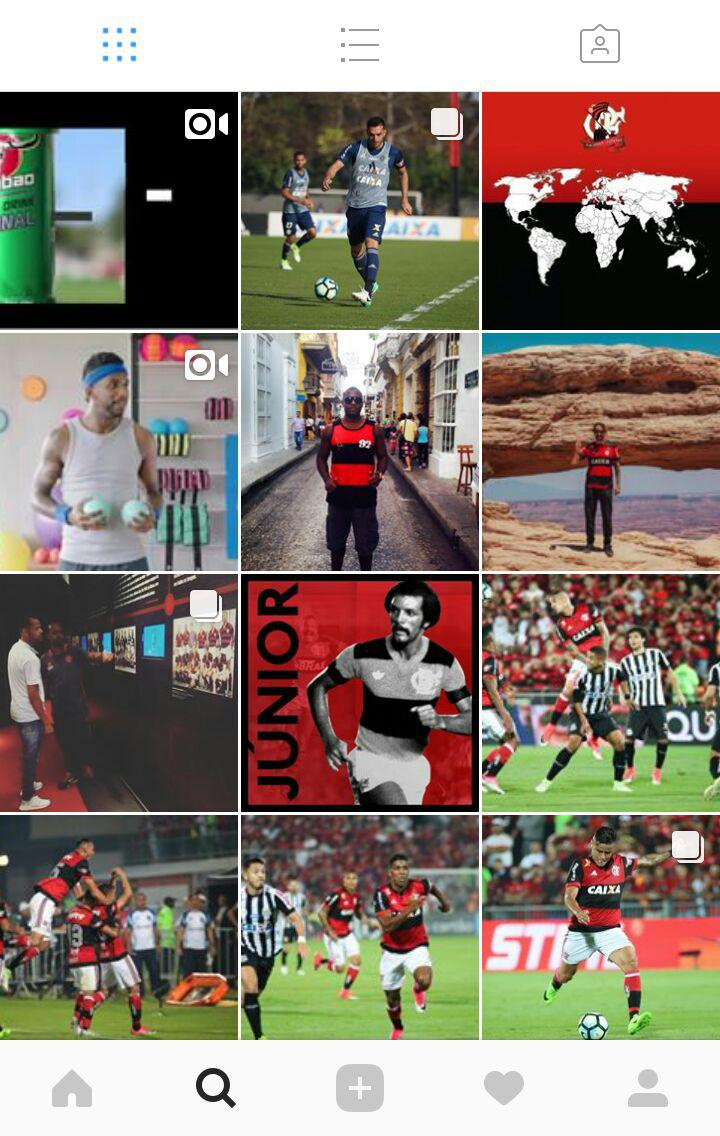
\includegraphics[scale=0.4]{instag.jpg}
	\end{center}
	\legend{Fonte: Reprodução (perfil do \textit{Clube de Regatas Flamengo} no \textit{Instagram})}
\end{figure}

\chapter{Percepção de cores}

Sobre a percepção de cores, o sistema se preocupou com a acessibilidade de usuários com dificuldades em distinguir cores, pois usa um sistema de cores monocromáticas em sua ultima versão. Tendo enfoco em uma proposta em valorizar as fotos e vídeos publicados pelos usuários, porém, sem grandes mudanças na navegação.

\chapter{Análise segundo a Engenharia Cognitiva}

A engenharia cognitiva foi concebida por Donald Norman em 1986 como uma tentativa de aplicar conhecimentos de ciência cognitiva, psicologia cognitiva e fatores humanos ao design e construção de sistemas computacionais. 

\section{Problemas de mapeamento}

Nesse programa não tem problemas em mapeamento, pois o desenvolvedor aplicou no sistema uma forma interativa de comunicação humano computador para melhor entendimento do usuário. 

\section{Dificuldade de controle}

A aplicação se mostrou isenta deste parâmetro.

\section{Dificuldade de avaliação}

Não a problemas quanto à avaliação, pois o desenvolvedor procurou formas de \textit{Affordance} nas quais o usuário, pode tirar conclusões ao olhar com imagens ilustrativas como exemplo de \textit{Affordance} o botão "curtir", e "comentários" como na Figura \ref{curtir}.

\begin{figure}[htb]
	\caption{\label{curtir}Curtir e comentar}
	\begin{center}
		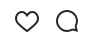
\includegraphics[scale=1]{instacurtir.jpg}
	\end{center}
	\legend{Fonte: Reprodução \textit{Instagram}}
\end{figure}

\chapter{Perspectiva de design: habilidades do designer}

O sistema foi bem elaborado e desenhando conforme as necessidades de usuários, está diretamente ligado no entendimento das funcionalidades, com ícones e legendas demonstrativas, e ajustes autoexplicativo, onde há facilidade de acesso e compreensão. Design inteligente e criativo com cores chamativas e não irritantes além da boa comodidade que o sistema apresenta.

\chapter{Coleta de dados: identificação das necessidades dos usuários}

Para realizar o levantamento de requisitos consultamos cerca de 30 pessoas sendo elas estudantes e servidores públicos, pedimos para que os mesmos respondesse um pequeno formulário que contém 5 questões subjetivas, sobre o uso do \textit{Instagram}.
Através dessa coleta de informações podemos perceber como os usuários que estão em contato com esse sistema, acham do sistema.

Através dessa coleta de dados. Obtivemos as seguintes informações:

O primeiro questionamento foi uma pergunta Objetiva, onde a pessoa foi questionada se a mesma aprova ou não o sistema.

\begin{figure}[htb]
	\caption{\label{gr01}Aprovação do sistema}
	\begin{center}
		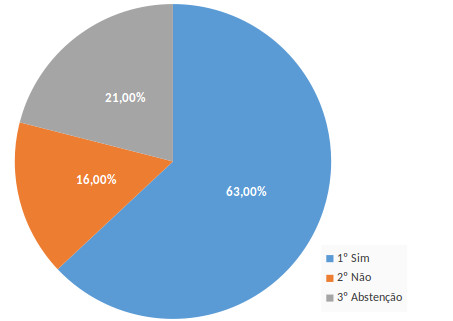
\includegraphics[scale=0.5]{graficos/01.jpg}
	\end{center}
\end{figure} 

Conforme vemos na Figura \ref{gr01}, 63\% dos entrevistados aprovam o sistema, enquanto que uma parcela de 16\% reprova e 21\% não souberam responder.

O segundo questionamento foi uma pergunta subjetiva, onde a pessoa foi questionada quais as vantagens de se utilizar o sistema.

\begin{figure}[h]
	\caption{\label{gr02}Vantagens da utilização do sistema}
	\begin{center}
		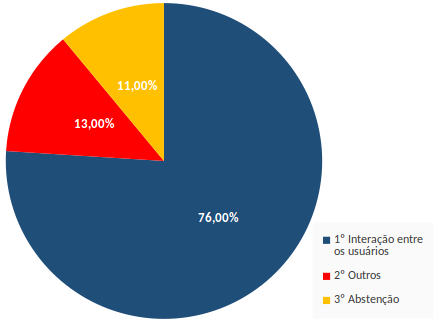
\includegraphics[scale=0.5]{graficos/02.jpg}
	\end{center}
\end{figure} 

Conforme na Figura \ref{gr02}, 76\% dos entrevistados apontam que a principal vantagem do sistema é a interação dos usúarios, ou seja, a aproximação entre internautas, por meio de fotos, videos, bate-papo e outras funcionalidades do sistema, enquanto 13\% responderam outra coisa e uma parcela de 11\% não souberam responder.

O terceiro questionamento foi uma pergunta subjetiva, onde a pessoa foi questionada quais as desvantagens de se utilizar o sistema.

\begin{figure}[h]
	\caption{\label{gr03}Desvantagens da utilização do sistema}
	\begin{center}
		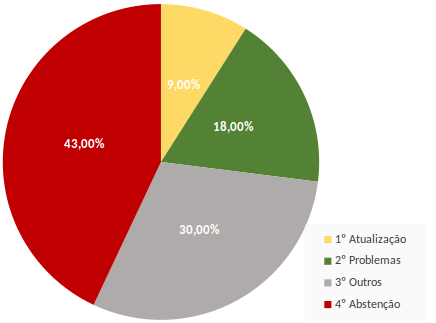
\includegraphics[scale=0.5]{graficos/03.jpg}
	\end{center}
\end{figure}

Conforme a Figura \ref{gr03}, 9\% dos entrevistados apontam como desvantagens do sistema, a  de atualização, para esses usuários o sistema é bom, mas falta acrescentar mais funcionalidades, 18\% apontaram que uma desvantagem seja problemas de conexão com a internet, 30\% responderam outros problemas e 43\% não souberam responder.

A quarto questionamento foi uma pergunta objetiva, onde a pessoa foi questionada se a mesma acredita que o sistema aqui apresentado, cumpre bem os seus deveres.

\begin{figure}[h]
	\caption{\label{gr04}O sistema cumpre bem o que promete}
	\begin{center}
		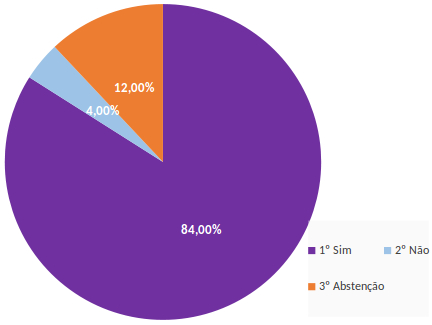
\includegraphics[scale=0.5]{graficos/04.jpg}
	\end{center}
\end{figure}

De acordo com a Figura \ref{gr04}, 84\% dos entrevistados acredita que o sistema cumpre bem os seus deveres, enquanto uma parcela de 4\% acha que não cumprem e 12\% não souberam responder.

O último questionamento foi uma pergunta objetiva, onde a pessoa foi questionada se a mesma acredita que o sistema fornece uma boa interação usuário-sistema. Isto é o senhor (o usuário) consegue compreender o \textit{Instagram}.

\begin{figure}[h]
	\caption{\label{gr05}Interação usuário sistema}
	\begin{center}
		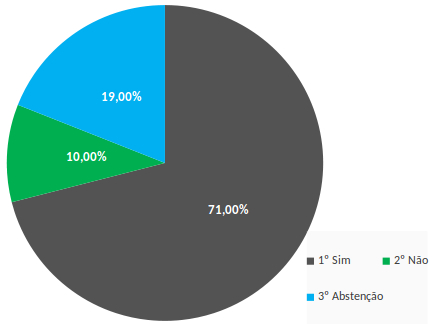
\includegraphics[scale=0.5]{graficos/05.jpg}
	\end{center}
\end{figure}

% ---
% Finaliza a parte no bookmark do PDF
% para que se inicie o bookmark na raiz
% e adiciona espaço de parte no Sumário
% ---
\phantompart

% ---
% Conclusão
% ---
\chapter*[Conclusão]{Conclusão}
\addcontentsline{toc}{chapter}{Conclusão}

Por conseguinte, no contexto atual em que o aplicativo \textit{Instagram} se encontra é perceptível a gigantesca evolução desde sua criação até os dias atuais no qual nos é contemplada a sua última versão. Podemos notar que a formula da rede social obteve sucesso no âmbito de interação com o usuário e isso vem aumentando a medida que a aplicação se torna mais acessível no meio social.

Percebemos então que o que poderia ser levado em consideração no quesito evolução, seria a plataforma. A mesma tem limitado bastante a experiência do usuário que espera que ela seja o mais semelhante com o aplicativo móvel possível.

Nos resta então agradecer pela oportunidade que nos foi dada de conhecer a área da Interação Humano-Computador, bem como agradecer o Docente pela paciência, disposição e compreensão no decorrer da disciplina. Com certeza o conteúdo da disciplina fez com que nós, Discentes, voltemos os olhares pra a IHC.

% ----------------------------------------------------------
% ELEMENTOS PÓS-TEXTUAIS
% ----------------------------------------------------------
\postextual

% ----------------------------------------------------------
% Referências bibliográficas
% ----------------------------------------------------------
\bibliography{abntex2-modelo-references}

% ----------------------------------------------------------
% Anexos
% ----------------------------------------------------------



%---------------------------------------------------------------------
% INDICE REMISSIVO
%---------------------------------------------------------------------

\phantompart

\printindex


\end{document}
